% =====================================================================
%  main.tex — plik główny pracy dyplomowej
%
%  Kolejność \include'ów poniżej to szkielet pracy wg wymogów wydziału
%  (strony wstępne -> wstęp -> rozdziały -> podsumowanie -> bibliografia
%  i dodatki). Rozdziały piszesz w plikach sections/ i podpinasz je
%  w odpowiednim miejscu tej listy. Numerki w nazwach plików (10-, 20-,
%  40-...) to porządek dla ludzi — LaTeX bierze kolejność z tej listy.
% =====================================================================
\documentclass[12pt]{article} % WYMOGI: 12pt

% Preambuła (pakiety, fonty, bibliografia) siedzi w core/packages.tex,
% dane pracy (temat, autor, promotor...) i makra — w core/macros.tex.
% =====================================================================
%  core/packages.tex — preambuła: pakiety, fonty, ustawienia globalne
%
%  Komentarz "WYMOGI" oznacza wartości narzucone przez wymagania
%  edytorskie wydziału — nie zmieniaj ich bez konsultacji z promotorem.
%  Kolejność ładowania też nie jest dowolna (np. unicode-math PO
%  fontspec, hyperref prawie na końcu) — przy przestawianiu czytaj
%  komentarze.
% =====================================================================

% --- 1. Podstawowa konfiguracja i język ---
\usepackage[a4paper, top=2.5cm, bottom=2.5cm, left=3.5cm, right=2cm]{geometry}
% WYMOGI: marginesy. Lewy 3,5 cm jest większy, bo tam strona schodzi pod oprawę.
\usepackage{indentfirst}
% Wcięcie także w pierwszym akapicie po nagłówku — polska konwencja typograficzna.
\usepackage[polish]{babel}
% Polskie napisy ("Rysunek", "Tabela", "Spis treści"...) i dzielenie wyrazów.
% W XeLaTeX używamy babel, a NIE pakietu 'polski' — tamten jest dla pdfLaTeX.

% --- 2. Fonty i matematyka (XeLaTeX) ---
% fontspec/unicode-math działają tylko pod XeLaTeX/LuaLaTeX — stąd -pdfxe w compile.sh.
\usepackage{mathtools} % nadzbiór amsmath (środowiska matematyczne)
\usepackage{amssymb}
\usepackage{amsthm}
\usepackage{fontspec}
\usepackage{unicode-math} % to musi być PO fontspec i amsmath

% Domyślny krój: Latin Modern. Teoretycznie powinien to być Times New Roman, jednak na
% linuxie jego instalcja jest problematyczna, a LM jest bardzo podobny i w pełni darmowy;
\setmainfont{Latin Modern Roman}
\setsansfont{Latin Modern Sans}

% Mono (kod źródłowy): Latin Modern Mono nie ma znaków indeksów dolnych (₀₁),
% więc bierzemy DejaVu Sans Mono — pełne pokrycie znaków, standard w Linuksie.
% Nie masz DejaVu? Tu wchodzi np. "FreeMono" albo "Courier New".
\setmonofont{DejaVu Sans Mono}[
	Scale=MatchLowercase,
	%FakeBold=1.0, % emulacja pogrubienia dla kodu
]

\setmathfont{Latin Modern Math} % wymagane przy unicode-math

% --- 3. Grafika i kolory ---
\usepackage{graphicx}          % \includegraphics — obrazki PNG/JPG/PDF
\usepackage{wrapfig}           % tekst opływający rysunek
\usepackage[section]{placeins} % rysunki nie uciekają poza swoją sekcję
\usepackage{float}             % opcja [H] = "dokładnie tutaj, nie kombinuj"
\usepackage{tikz}              % rysunki wektorowe w kodzie (przykład: 50-impl.tex)
\usepackage{pgfplots}          % wykresy w TikZ-u
\pgfplotsset{compat=1.18}

% \usepackage[inkscapeformat=png]{svg}
% ^ Odkomentuj, jeśli chcesz wstawiać .svg. Wymaga zainstalowanego Inkscape
%   (konwersja dzieje się przy kompilacji). Bez .svg w pracy — nie włączaj.
%   użyj wtedy \includesvg{pathdopliku}

% --- 4. Tabele i listy ---
\usepackage{paralist}  % kompaktowe listy (compactitem i spółka)
\usepackage{enumerate} % własne etykiety w \begin{enumerate}[...]
\usepackage{multirow}  % komórka na kilka wierszy
\usepackage{multicol}  % kilka łamów w obrębie strony
\usepackage{tabulary}  % tabele z zawijaniem tekstu do szerokości
\usepackage{ragged2e}  % \justify i spółka (używane na stronie tytułowej)
\usepackage{makecell}  % wielolinijkowe komórki \makecell{...}
\usepackage{tocloft}   % styl spisu treści (szerokość kolumny numerów itd.)

% --- 5. Kod i algorytmy ---
\usepackage{minted}
% minted koloruje składnię przez ZEWNĘTRZNY program pygmentize, dlatego:
%  a) musi być zainstalowany (pip install Pygments; test: pygmentize -V),
%  b) kompilacja musi iść z -shell-escape — compile.sh już to robi.
\usepackage[ruled, vlined]{algorithm2e} % pseudokod (przykład: 50-impl.tex)

% --- 6. Bibliografia (biblatex) ---
\usepackage[nottoc]{tocbibind}
% Spisy i bibliografia wchodzą do spisu treści
\usepackage[
	sorting=none,       % numery [1], [2]... w kolejności CYTOWANIA, nie alfabetycznie
	style=numeric-comp, % styl numerowany, [3–6] zamiast [3,4,5,6]
	maxbibnames=3,      % przy 4+ autorach w bibliografii pojawia się "i in."
	minbibnames=3
]{biblatex}
\addbibresource{bibl.bib} % baza źródeł; klucze cytujesz przez \cite{klucz}
\DefineBibliographyStrings{polish}{
	andothers = {i~in\adddot} % polskie "i in." zamiast "et al."
}

% --- 7. Różne ---
\usepackage{siunitx} % jednostki i liczby: \qty{9.81}{m/s^2} -> "9,81 m/s²"
\linespread{1.5}     % WYMOGI: interlinia 1,5
\parindent=1cm       % WYMOGI: wcięcie akapitowe
\setlength{\cftfignumwidth}{4em} % tocloft: miejsce na numery w spisie treści

% Numeracja wewnątrz rozdziałów: wzór (3.1), rysunek 3.1 itd.
\numberwithin{equation}{section}
\numberwithin{figure}{section}
\counterwithin{figure}{section}

% Polskie nazwy algorytmów ("Algorytm 1"; spis: "Spis algorytmów")
\SetAlgorithmName{Algorytm}{algorytm}{Spis algorytmów}

% Biblioteki TikZ. Dokładanie "na zapas" spowalnia kompilację —
% dopisuj, gdy faktycznie czegoś brakuje.
\usetikzlibrary{
	automata, shapes.multipart, positioning, arrows.meta,
	shadows, fit, shapes.geometric, calc, patterns
}

% --- 8. Pakiety ingerujące w PDF (ładować na końcu!) ---
\usepackage{pdfpages} % \includepdf — np. wklejenie karty dyplomowej PDF (0-head.tex)

\usepackage[colorlinks, plainpages=false, pdfpagelabels, naturalnames=true]{hyperref}
\hypersetup{
	linkcolor={black!50!black}, % odnośniki wewnętrzne
	citecolor={blue!50!black}, % cytowania: przygaszony niebieski
	urlcolor={blue!80!black}   % adresy www: niebieski
}

% --- Koniec preambuły ---

% =====================================================================
%  core/macros.tex — dane pracy i drobne makra wspólne
%  (Plik dołączany z main.tex przez \input.)
% =====================================================================

% ---------------------------------------------------------------------
%  DANE PRACY — uzupełnij poniższe makra. Wpisujesz raz, strona tytułowa
%  (sections/0-head.tex) i Summary aktualizują się same.
% ---------------------------------------------------------------------

% Typ pracy: inżynierska albo magisterska.
\newcommand{\thesisType}{PRACA DYPLOMOWA INŻYNIERSKA}

% Streszczenie po angielsku (trafia na osobną stronę po stronie tytułowej).
\newcommand{\summaryEN}{
  TUTAJ WPISZ SUMMARY PRACY PO ANG

Lorem ipsum dolor sit amet, consectetur adipiscing elit. Nunc in vehicula est. Proin a justo sagittis, interdum nisl nec, viverra dolor. Etiam at porttitor justo. Ut ut enim nibh. Donec tellus turpis, convallis pulvinar urna sit amet, placerat dignissim felis. Cras tempor eget nunc eu sagittis. Vivamus eget nunc dignissim, lobortis enim quis, sagittis urna. Aenean eget erat dapibus, fermentum arcu sed, lacinia augue. Maecenas velit enim, mollis sed pharetra ac, porta id libero.

  }

\newcommand{\topicPL}{Temat pracy po polsku}
\newcommand{\topicEN}{Temat pracy po angielsku}

\newcommand{\thesisAuthor}{TWOJE IMIĘ I NAZWISKO}
\newcommand{\thesisDate}{BIAŁYSTOK 20XX ROK}

\newcommand{\promotor}{prof. dr hab. inż. PROMOTOR}

% ---------------------------------------------------------------------
%  Rozdziały bez numeru (Wstęp, Podsumowanie, Dodatki) robi się ręcznie
%  dwiema linijkami — i dokładnie tak trzeba, bo \section* sam z siebie
%  nie trafia do spisu treści:
%
%      \section*{Wstęp}
%      \addcontentsline{toc}{section}{Wstęp}
%
%  hyperref (załadowany w packages.tex) zakotwicza odnośnik w miejscu
%  wpisu, więc klik w spisie treści prowadzi dokładnie w to miejsce.
%  Zwykłe, numerowane rozdziały: po prostu \section{Tytuł}.
% ---------------------------------------------------------------------

% Nazwy używane pośrednio przez pakiet listings (a więc i przez minted):
% prefiks podpisu pod listingiem ("Listing 3: ...") oraz tytuł spisu listingów.
\renewcommand{\listingscaption}{Listing}
\renewcommand{\listoflistingscaption}{Spis listingów}


\begin{document}

% --- Strony wstępne (układ wydziałowy — nie przemeblowywać) ---
% =====================================================================
%  sections/0-head.tex — strony wstępne: tytułowa, temat po angielsku,
%  Summary, spis treści.
%
%  Układ (rozmieszczenie, odstępy, rozmiary czcionek) jest pod wymagania
%  wydziału — traktuj jak mebel na stałe. Twoja część to makra z
%  core/macros.tex: \thesisType, \topicPL, \thesisAuthor, \promotor,
%  \thesisDate i \summaryEN. Strony wstępne są nienumerowane
%  (\thispagestyle{empty}); numeracja „1" zaczyna się od Wstępu.
% =====================================================================
\begin{center}
	\fontsize{20pt}{20pt}\selectfont
	\textbf{POLITECHNIKA BIAŁOSTOCKA}
	\vspace{1.0cm}

	\fontsize{14pt}{14pt}\selectfont
	\textbf{WYDZIAŁ INFORMATYKI}
	\vspace{4.0cm}

	\fontsize{18pt}{18pt}\selectfont
	\thesisType
	\fontsize{16pt}{16pt}\selectfont

	\vspace{0.8cm}

	\fontsize{14pt}{14pt}\selectfont

	\vspace{1.6cm}

	TEMAT: \topicPL

	\vspace{1.6cm}

\end{center}
\fontsize{14pt}{14pt}\selectfont

\vspace{3,4cm}

\begin{flushright}
	\begin{tabular}{rl}
		WYKONAWCA: & \thesisAuthor \\
		           &               \\
	\end{tabular}
	\vfill
\end{flushright}

\begin{flushleft}
	\begin{tabular}{rl}
		OPIEKUN PRACY DYPLOMOWEJ: & \promotor \\
		                          &           \\
	\end{tabular}
\end{flushleft}

\vspace{2cm}

\begin{center}
	\textbf{\thesisDate}
\end{center}

\thispagestyle{empty}

\pagebreak\ \thispagestyle{empty}

\noindent Subject of diploma thesis:

\noindent \topicEN

\thispagestyle{empty}
\begin{center}
	\Large
	\textbf{Summary}

	\normalsize
	\justify
	\summaryEN
\end{center}


\pagebreak

\thispagestyle{empty}
% Karta dyplomowa od dziekanatu (PDF)? Odkomentuj — pakiet pdfpages jest
% już załadowany w preambule:
%    \includepdf[pages=2]{KartaDyplomowa.pdf}
\thispagestyle{empty}

\pagestyle{empty}
\pagebreak

\normalsize

\pagebreak
% Spis treści buduje się sam: wpisy biorą się z \section i z ręcznych
% \addcontentsline (Wstęp, Podsumowanie, Dodatki).
\addtocontents{toc}{\protect\thispagestyle{empty}}
\tableofcontents
\pagebreak
 % strona tytułowa, temat po angielsku, Summary, spis treści

% --- Treść pracy ---
\pagestyle{plain}

% AUTOTUTORIAL — rozdział "jak używać tego szablonu".
% PRZED ODDANIEM PRACY usuń (lub zakomentuj) poniższą linię.
% =====================================================================
%  sections/05-tutorial.tex — AUTOTUTORIAL
%
%  Rozdział, w którym szablon opisuje sam siebie — na przykładach, które
%  sam demonstruje. Dołączany z main.tex.
%
%  PRZED ODDANIEM PRACY: usuń (lub zakomentuj) w main.tex linię
%      % =====================================================================
%  sections/05-tutorial.tex — AUTOTUTORIAL
%
%  Rozdział, w którym szablon opisuje sam siebie — na przykładach, które
%  sam demonstruje. Dołączany z main.tex.
%
%  PRZED ODDANIEM PRACY: usuń (lub zakomentuj) w main.tex linię
%      % =====================================================================
%  sections/05-tutorial.tex — AUTOTUTORIAL
%
%  Rozdział, w którym szablon opisuje sam siebie — na przykładach, które
%  sam demonstruje. Dołączany z main.tex.
%
%  PRZED ODDANIEM PRACY: usuń (lub zakomentuj) w main.tex linię
%      \include{sections/05-tutorial}
%  i zerknij na listę kontrolną z ostatniej podsekcji tego pliku.
% =====================================================================

\section*{Autotutorial, czyli szablon o sobie samym}
\addcontentsline{toc}{section}{Autotutorial, czyli szablon o sobie samym}
% ^ Właśnie obejrzałeś ręczny patent na rozdział bez numeru, ale z wpisem
%   w spisie treści. Tak samo zbudowany jest Wstęp, Podsumowanie i Dodatki
%   (a Numerowany zwykły rozdział dostajesz przez \section{Tytuł}).

Ten rozdział jest tu po to, żebyś TY\footnote{twój LLM} nie czytał dokumentacji pakietów
o drugiej w nocy. Każdy element, o którym mowa, powinien być gdzieś w szablonie
użyty na żywo — podglądaj PDF obok źródła, to najszybsza forma nauki.

\subsection*{Kompilacja}

Cały proces zamknięty jest w \verb|compile.sh|:

\begin{verbatim}
latexmk -bibtex -shell-escape -interaction=nonstopmode -pdfxe main.tex
\end{verbatim}

latexmk sam ustala, ile przebiegów potrzeba (spis treści i odsyłacze
\verb|\ref| „łapią" numery dopiero po drugim podejściu).
Dwie flagi zasługują na wyjaśnienie:
\begin{itemize}
	\item \verb|-shell-escape| — pakiet minted (kolorowanie kodu) odpala
	      zewnętrzny program \texttt{pygmentize}, a LaTeX domyślnie blokuje
	      uruchamianie obcych programów. Flaga jest zgodą. Jak pygmentize
	      nie masz: \verb|pip install Pygments|.
	\item \verb|-pdfxe| — silnik XeLaTeX, bo preambuła używa fontspec
	      i unicode-math (fonty systemowe, polskie znaki bez sztuczek).
\end{itemize}

Gdy kompilacja padnie: przeczytaj komunikat — pierwszy błąd się liczy,
kolejne to zwykle echa. Jeśli log nic sensownego nie mówi, usuń pliki
pomocnicze (\verb|latexmk -c|) i skompiluj od nowa.

\subsection*{Mapa projektu}

\begin{table}[H]
	\centering
	\caption{Mapa projektu. A tak wygląda tabela: środowisko
		\texttt{table} z podpisem \texttt{\textbackslash caption}
		i \texttt{\textbackslash label} zaraz po nim.}
	\label{tab:mapa-projektu}
	\begin{tabular}{|l|p{8.5cm}|}
		\hline
		\textbf{Plik}              & \textbf{Rola}                                  \\
		\hline
		\texttt{main.tex}          & szkielet: kolejność rozdziałów                 \\
		\texttt{core/packages.tex} & preambuła: pakiety, fonty, bibliografia        \\
		\texttt{core/macros.tex}   & dane pracy (temat, autor, promotor...) i makra \\
		\texttt{sections/*.tex}    & rozdziały — tu się pisze                       \\
		\texttt{img/}              & obrazki                                        \\
		\texttt{bibl.bib}          & baza źródeł do \texttt{\textbackslash cite}    \\
		\texttt{compile.sh}        & kompilacja jednym poleceniem                   \\
		\hline
	\end{tabular}
\end{table}

\subsection*{Dane pracy}

Temat (PL i EN), autor, promotor, data, typ pracy i angielskie Summary
to makra w \verb|core/macros.tex|. Rozkład strony tytułowej
(\verb|sections/0-head.tex|) odpowiada wymaganiom wydziału.

\subsection*{Pisanie rozdziałów}

\begin{itemize}
	\item \verb|\section{Tytuł}| — numerowany rozdział;
	\item rozdział bez numeru, ale w spisie treści (Wstęp, Podsumowanie,
	      Dodatki):
	      \verb|\section*{Wstęp}| plus \verb|\addcontentsline{toc}{section}{Wstęp}|;
	\item \verb|\subsection|, \verb|\subsubsection| — podział wewnątrz rozdziału.
\end{itemize}

Nowy rozdział to zwykle nowy plik w \verb|sections/| podpięty
\verb|\include| w \verb|main.tex| w odpowiednim miejscu listy.

\subsection*{Elementy składowe — gdzie zobaczyć na żywo}

Szablon zawiera działające przykłady wszystkiego, co typowej pracy
potrzebne:
\begin{itemize}
	\item rysunek kaczki z podpisem i źródłem: rozdział Wprowadzenie
	      (rysunek \ref{fig:duck} na str. \pageref{fig:duck};
	      tak, powtarzając 17 raz, to JEST KACZKA.
	\item tabela: badania eksperymentalne (tabela \ref{tab:xor-dataset}),
	\item wzór z odsyłaczem „(str. X)": implementacja, równanie
	      (\ref{eq:indeksliczenie}),
	\item listing z kolorowaniem składni (Python i Rust): analiza
	      istniejących rozwiązań oraz implementacja,
	\item algorytm w pseudokodzie i obrazek rysowany w TikZ-u: implementacja
	      (algorytm \ref{alg:tensor-iter}),
	\item cytowania \verb|\cite{...}|: analiza istniejących rozwiązań
	      i bibliografia na końcu dokumentu.
\end{itemize}

Żelazne zasady, które oszczędzają nerwów: \verb|\label| zawsze PO
\verb|\caption|, a każdy
rysunek i tabela dostają w podpisie źródło — „Źródło: opracowanie własne"
też jest źródłem.

\subsection*{Bibliografia}

Źródła dopisujesz do \verb|bibl.bib| i cytujesz \verb|\cite{klucz}| (wiele
naraz: \verb|\cite{a, b, c}|). Numery w bibliografii nadają się same, po
kolei cytowania — takie jest ustawienie \verb|sorting=none| w preambule.
Strony internetowe cytujemy z datą dostępu
(\verb|note = {[Dostęp dnia: 01.04.2025]}|). W \verb|bibl.bib| czeka po
jednym przykładzie każdego typu wpisu — od artykułu po stronę www.

\subsection*{Lista kontrolna przed oddaniem}

\begin{itemize}
	\item w \verb|main.tex| usunięta linia dołączająca ten tutorial,
	\item makra w \verb|core/macros.tex|: temat PL/EN, autor, promotor,
	      data, typ pracy, \textit{Summary} po angielsku,
	\item każdy rysunek i tabela mają podpis ze źródłem, ORAZ wspominasz
	      o nich w tekście (np. „na rysunku \ref{fig:duck} widać kaczkę. Naprawdę, to kaczka."),
	\item \verb|\label| po \verb|\caption| — odsyłacze mówią prawdę,
	\item dodatek o archiwum plików opisuje to, co faktycznie tam jest,
	\item końcowa kompilacja: log bez czerwonych linii, spis treści zgodny
	      z rzeczywistością,
	\item ortografia. Promotor czyta. Naprawdę.
\end{itemize}

Powodzenia.

%  i zerknij na listę kontrolną z ostatniej podsekcji tego pliku.
% =====================================================================

\section*{Autotutorial, czyli szablon o sobie samym}
\addcontentsline{toc}{section}{Autotutorial, czyli szablon o sobie samym}
% ^ Właśnie obejrzałeś ręczny patent na rozdział bez numeru, ale z wpisem
%   w spisie treści. Tak samo zbudowany jest Wstęp, Podsumowanie i Dodatki
%   (a Numerowany zwykły rozdział dostajesz przez \section{Tytuł}).

Ten rozdział jest tu po to, żebyś TY\footnote{twój LLM} nie czytał dokumentacji pakietów
o drugiej w nocy. Każdy element, o którym mowa, powinien być gdzieś w szablonie
użyty na żywo — podglądaj PDF obok źródła, to najszybsza forma nauki.

\subsection*{Kompilacja}

Cały proces zamknięty jest w \verb|compile.sh|:

\begin{verbatim}
latexmk -bibtex -shell-escape -interaction=nonstopmode -pdfxe main.tex
\end{verbatim}

latexmk sam ustala, ile przebiegów potrzeba (spis treści i odsyłacze
\verb|\ref| „łapią" numery dopiero po drugim podejściu).
Dwie flagi zasługują na wyjaśnienie:
\begin{itemize}
	\item \verb|-shell-escape| — pakiet minted (kolorowanie kodu) odpala
	      zewnętrzny program \texttt{pygmentize}, a LaTeX domyślnie blokuje
	      uruchamianie obcych programów. Flaga jest zgodą. Jak pygmentize
	      nie masz: \verb|pip install Pygments|.
	\item \verb|-pdfxe| — silnik XeLaTeX, bo preambuła używa fontspec
	      i unicode-math (fonty systemowe, polskie znaki bez sztuczek).
\end{itemize}

Gdy kompilacja padnie: przeczytaj komunikat — pierwszy błąd się liczy,
kolejne to zwykle echa. Jeśli log nic sensownego nie mówi, usuń pliki
pomocnicze (\verb|latexmk -c|) i skompiluj od nowa.

\subsection*{Mapa projektu}

\begin{table}[H]
	\centering
	\caption{Mapa projektu. A tak wygląda tabela: środowisko
		\texttt{table} z podpisem \texttt{\textbackslash caption}
		i \texttt{\textbackslash label} zaraz po nim.}
	\label{tab:mapa-projektu}
	\begin{tabular}{|l|p{8.5cm}|}
		\hline
		\textbf{Plik}              & \textbf{Rola}                                  \\
		\hline
		\texttt{main.tex}          & szkielet: kolejność rozdziałów                 \\
		\texttt{core/packages.tex} & preambuła: pakiety, fonty, bibliografia        \\
		\texttt{core/macros.tex}   & dane pracy (temat, autor, promotor...) i makra \\
		\texttt{sections/*.tex}    & rozdziały — tu się pisze                       \\
		\texttt{img/}              & obrazki                                        \\
		\texttt{bibl.bib}          & baza źródeł do \texttt{\textbackslash cite}    \\
		\texttt{compile.sh}        & kompilacja jednym poleceniem                   \\
		\hline
	\end{tabular}
\end{table}

\subsection*{Dane pracy}

Temat (PL i EN), autor, promotor, data, typ pracy i angielskie Summary
to makra w \verb|core/macros.tex|. Rozkład strony tytułowej
(\verb|sections/0-head.tex|) odpowiada wymaganiom wydziału.

\subsection*{Pisanie rozdziałów}

\begin{itemize}
	\item \verb|\section{Tytuł}| — numerowany rozdział;
	\item rozdział bez numeru, ale w spisie treści (Wstęp, Podsumowanie,
	      Dodatki):
	      \verb|\section*{Wstęp}| plus \verb|\addcontentsline{toc}{section}{Wstęp}|;
	\item \verb|\subsection|, \verb|\subsubsection| — podział wewnątrz rozdziału.
\end{itemize}

Nowy rozdział to zwykle nowy plik w \verb|sections/| podpięty
\verb|\include| w \verb|main.tex| w odpowiednim miejscu listy.

\subsection*{Elementy składowe — gdzie zobaczyć na żywo}

Szablon zawiera działające przykłady wszystkiego, co typowej pracy
potrzebne:
\begin{itemize}
	\item rysunek kaczki z podpisem i źródłem: rozdział Wprowadzenie
	      (rysunek \ref{fig:duck} na str. \pageref{fig:duck};
	      tak, powtarzając 17 raz, to JEST KACZKA.
	\item tabela: badania eksperymentalne (tabela \ref{tab:xor-dataset}),
	\item wzór z odsyłaczem „(str. X)": implementacja, równanie
	      (\ref{eq:indeksliczenie}),
	\item listing z kolorowaniem składni (Python i Rust): analiza
	      istniejących rozwiązań oraz implementacja,
	\item algorytm w pseudokodzie i obrazek rysowany w TikZ-u: implementacja
	      (algorytm \ref{alg:tensor-iter}),
	\item cytowania \verb|\cite{...}|: analiza istniejących rozwiązań
	      i bibliografia na końcu dokumentu.
\end{itemize}

Żelazne zasady, które oszczędzają nerwów: \verb|\label| zawsze PO
\verb|\caption|, a każdy
rysunek i tabela dostają w podpisie źródło — „Źródło: opracowanie własne"
też jest źródłem.

\subsection*{Bibliografia}

Źródła dopisujesz do \verb|bibl.bib| i cytujesz \verb|\cite{klucz}| (wiele
naraz: \verb|\cite{a, b, c}|). Numery w bibliografii nadają się same, po
kolei cytowania — takie jest ustawienie \verb|sorting=none| w preambule.
Strony internetowe cytujemy z datą dostępu
(\verb|note = {[Dostęp dnia: 01.04.2025]}|). W \verb|bibl.bib| czeka po
jednym przykładzie każdego typu wpisu — od artykułu po stronę www.

\subsection*{Lista kontrolna przed oddaniem}

\begin{itemize}
	\item w \verb|main.tex| usunięta linia dołączająca ten tutorial,
	\item makra w \verb|core/macros.tex|: temat PL/EN, autor, promotor,
	      data, typ pracy, \textit{Summary} po angielsku,
	\item każdy rysunek i tabela mają podpis ze źródłem, ORAZ wspominasz
	      o nich w tekście (np. „na rysunku \ref{fig:duck} widać kaczkę. Naprawdę, to kaczka."),
	\item \verb|\label| po \verb|\caption| — odsyłacze mówią prawdę,
	\item dodatek o archiwum plików opisuje to, co faktycznie tam jest,
	\item końcowa kompilacja: log bez czerwonych linii, spis treści zgodny
	      z rzeczywistością,
	\item ortografia. Promotor czyta. Naprawdę.
\end{itemize}

Powodzenia.

%  i zerknij na listę kontrolną z ostatniej podsekcji tego pliku.
% =====================================================================

\section*{Autotutorial, czyli szablon o sobie samym}
\addcontentsline{toc}{section}{Autotutorial, czyli szablon o sobie samym}
% ^ Właśnie obejrzałeś ręczny patent na rozdział bez numeru, ale z wpisem
%   w spisie treści. Tak samo zbudowany jest Wstęp, Podsumowanie i Dodatki
%   (a Numerowany zwykły rozdział dostajesz przez \section{Tytuł}).

Ten rozdział jest tu po to, żebyś TY\footnote{twój LLM} nie czytał dokumentacji pakietów
o drugiej w nocy. Każdy element, o którym mowa, powinien być gdzieś w szablonie
użyty na żywo — podglądaj PDF obok źródła, to najszybsza forma nauki.

\subsection*{Kompilacja}

Cały proces zamknięty jest w \verb|compile.sh|:

\begin{verbatim}
latexmk -bibtex -shell-escape -interaction=nonstopmode -pdfxe main.tex
\end{verbatim}

latexmk sam ustala, ile przebiegów potrzeba (spis treści i odsyłacze
\verb|\ref| „łapią" numery dopiero po drugim podejściu).
Dwie flagi zasługują na wyjaśnienie:
\begin{itemize}
	\item \verb|-shell-escape| — pakiet minted (kolorowanie kodu) odpala
	      zewnętrzny program \texttt{pygmentize}, a LaTeX domyślnie blokuje
	      uruchamianie obcych programów. Flaga jest zgodą. Jak pygmentize
	      nie masz: \verb|pip install Pygments|.
	\item \verb|-pdfxe| — silnik XeLaTeX, bo preambuła używa fontspec
	      i unicode-math (fonty systemowe, polskie znaki bez sztuczek).
\end{itemize}

Gdy kompilacja padnie: przeczytaj komunikat — pierwszy błąd się liczy,
kolejne to zwykle echa. Jeśli log nic sensownego nie mówi, usuń pliki
pomocnicze (\verb|latexmk -c|) i skompiluj od nowa.

\subsection*{Mapa projektu}

\begin{table}[H]
	\centering
	\caption{Mapa projektu. A tak wygląda tabela: środowisko
		\texttt{table} z podpisem \texttt{\textbackslash caption}
		i \texttt{\textbackslash label} zaraz po nim.}
	\label{tab:mapa-projektu}
	\begin{tabular}{|l|p{8.5cm}|}
		\hline
		\textbf{Plik}              & \textbf{Rola}                                  \\
		\hline
		\texttt{main.tex}          & szkielet: kolejność rozdziałów                 \\
		\texttt{core/packages.tex} & preambuła: pakiety, fonty, bibliografia        \\
		\texttt{core/macros.tex}   & dane pracy (temat, autor, promotor...) i makra \\
		\texttt{sections/*.tex}    & rozdziały — tu się pisze                       \\
		\texttt{img/}              & obrazki                                        \\
		\texttt{bibl.bib}          & baza źródeł do \texttt{\textbackslash cite}    \\
		\texttt{compile.sh}        & kompilacja jednym poleceniem                   \\
		\hline
	\end{tabular}
\end{table}

\subsection*{Dane pracy}

Temat (PL i EN), autor, promotor, data, typ pracy i angielskie Summary
to makra w \verb|core/macros.tex|. Rozkład strony tytułowej
(\verb|sections/0-head.tex|) odpowiada wymaganiom wydziału.

\subsection*{Pisanie rozdziałów}

\begin{itemize}
	\item \verb|\section{Tytuł}| — numerowany rozdział;
	\item rozdział bez numeru, ale w spisie treści (Wstęp, Podsumowanie,
	      Dodatki):
	      \verb|\section*{Wstęp}| plus \verb|\addcontentsline{toc}{section}{Wstęp}|;
	\item \verb|\subsection|, \verb|\subsubsection| — podział wewnątrz rozdziału.
\end{itemize}

Nowy rozdział to zwykle nowy plik w \verb|sections/| podpięty
\verb|\include| w \verb|main.tex| w odpowiednim miejscu listy.

\subsection*{Elementy składowe — gdzie zobaczyć na żywo}

Szablon zawiera działające przykłady wszystkiego, co typowej pracy
potrzebne:
\begin{itemize}
	\item rysunek kaczki z podpisem i źródłem: rozdział Wprowadzenie
	      (rysunek \ref{fig:duck} na str. \pageref{fig:duck};
	      tak, powtarzając 17 raz, to JEST KACZKA.
	\item tabela: badania eksperymentalne (tabela \ref{tab:xor-dataset}),
	\item wzór z odsyłaczem „(str. X)": implementacja, równanie
	      (\ref{eq:indeksliczenie}),
	\item listing z kolorowaniem składni (Python i Rust): analiza
	      istniejących rozwiązań oraz implementacja,
	\item algorytm w pseudokodzie i obrazek rysowany w TikZ-u: implementacja
	      (algorytm \ref{alg:tensor-iter}),
	\item cytowania \verb|\cite{...}|: analiza istniejących rozwiązań
	      i bibliografia na końcu dokumentu.
\end{itemize}

Żelazne zasady, które oszczędzają nerwów: \verb|\label| zawsze PO
\verb|\caption|, a każdy
rysunek i tabela dostają w podpisie źródło — „Źródło: opracowanie własne"
też jest źródłem.

\subsection*{Bibliografia}

Źródła dopisujesz do \verb|bibl.bib| i cytujesz \verb|\cite{klucz}| (wiele
naraz: \verb|\cite{a, b, c}|). Numery w bibliografii nadają się same, po
kolei cytowania — takie jest ustawienie \verb|sorting=none| w preambule.
Strony internetowe cytujemy z datą dostępu
(\verb|note = {[Dostęp dnia: 01.04.2025]}|). W \verb|bibl.bib| czeka po
jednym przykładzie każdego typu wpisu — od artykułu po stronę www.

\subsection*{Lista kontrolna przed oddaniem}

\begin{itemize}
	\item w \verb|main.tex| usunięta linia dołączająca ten tutorial,
	\item makra w \verb|core/macros.tex|: temat PL/EN, autor, promotor,
	      data, typ pracy, \textit{Summary} po angielsku,
	\item każdy rysunek i tabela mają podpis ze źródłem, ORAZ wspominasz
	      o nich w tekście (np. „na rysunku \ref{fig:duck} widać kaczkę. Naprawdę, to kaczka."),
	\item \verb|\label| po \verb|\caption| — odsyłacze mówią prawdę,
	\item dodatek o archiwum plików opisuje to, co faktycznie tam jest,
	\item końcowa kompilacja: log bez czerwonych linii, spis treści zgodny
	      z rzeczywistością,
	\item ortografia. Promotor czyta. Naprawdę.
\end{itemize}

Powodzenia.


% =====================================================================
%  Wstęp — bez numeru, ale z wpisem w spisie treści.
%  Dlatego ręcznie: \section* + \addcontentsline
% =====================================================================
\section*{Wstęp}
\addcontentsline{toc}{section}{Wstęp}

\setcounter{page}{1} % numeracja stron zaczyna się tutaj; strony wstępne nie są numerowane

% Lorem ipsum poniżej to wypełniacz. Jego używanie jest bardzo oryginalne.
Lorem ipsum dolor sit amet, consectetur adipiscing elit. Nunc in vehicula est. Proin a justo sagittis, interdum nisl nec, viverra dolor. Etiam at porttitor justo. Ut ut enim nibh. Donec tellus turpis, convallis pulvinar urna sit amet, placerat dignissim felis. Cras tempor eget nunc eu sagittis. Vivamus eget nunc dignissim, lobortis enim quis, sagittis urna. Aenean eget erat dapibus, fermentum arcu sed, lacinia augue. Maecenas velit enim, mollis sed pharetra ac, porta id libero.

Suspendisse non velit lobortis, pharetra lacus nec, efficitur massa. Morbi eu dictum libero. Donec tincidunt cursus nisi, a sodales magna fringilla eu. Curabitur fringilla bibendum magna ac commodo. Morbi a nibh nisl. Morbi blandit tortor vitae iaculis aliquet. Phasellus commodo tincidunt arcu, ut consequat mi maximus vel. Donec eleifend varius ligula, et rutrum massa iaculis a. Praesent augue libero, vehicula ac massa vel, pulvinar pulvinar mauris. Aliquam nec felis ornare, sodales est ut, consectetur magna. Duis imperdiet rhoncus aliquet.

Vivamus massa enim, mattis sed nunc in, lacinia sollicitudin augue. Duis facilisis sed risus vitae fringilla. Phasellus nec ipsum quam. Interdum et malesuada fames ac ante ipsum primis in faucibus. Sed sed tortor at tellus vehicula porttitor vitae eget massa. Suspendisse potenti. Pellentesque augue neque, finibus nec porttitor vel, tincidunt hendrerit tortor. Vestibulum ut augue leo.

Proin a velit porttitor, sodales erat ac, sodales ex. Nam maximus, magna sed pulvinar mattis, ante augue blandit urna, non ultricies nulla mi sed lacus. Aenean aliquam rutrum turpis quis commodo. Donec vel molestie risus, non euismod nibh. Donec a orci ut dui dignissim placerat quis vitae diam. Proin tempor nulla vitae elit lacinia pellentesque. Etiam pellentesque congue diam, eget bibendum lacus. Praesent mattis viverra efficitur. Cras interdum nisl turpis, vel efficitur ligula gravida quis. Sed at ultricies mauris. Quisque eget ipsum vitae metus ultrices tristique. Curabitur eleifend arcu a risus sagittis volutpat. In tincidunt elit vel gravida lobortis. Nulla et elementum eros, tincidunt rutrum quam.

Quisque at sollicitudin nisi, sit amet auctor lorem. Vestibulum sit amet nunc consequat, blandit mi id, aliquet magna. Suspendisse potenti. Cras convallis felis eget viverra porta. Vivamus placerat purus sagittis nunc tincidunt elementum. Interdum et malesuada fames ac ante ipsum primis in faucibus. Aliquam convallis feugiat lacus, a aliquet diam sagittis id.
        % Wstęp (bez numeru, w spisie treści)
% =====================================================================
%  Wprowadzenie — pierwszy rozdział numerowany: od tego miejsca LaTeX
%  numeruje rozdziały, a wzory/rysunki dostają numery z numerem
%  rozdziału (ustawienie \numberwithin{...}{section} w packages.tex).
%
%  Ten rozdział demonstruje wstawianie rysunków:
%  figure + includegraphics + caption + label + odsyłacze \ref (numer)
%  i \pageref (strona). 
% =====================================================================
\section{Wprowadzenie}

% Wzorcowy schemat rysunku: podpis z obowiązkowym źródłem, \label PO
% \caption (inaczej \ref pokaże złą liczbę).
% tak, poniższy rysunek definitywnie przedstawia kaczkę - przecież autor
% nie mógłby wstawić zdjęcia gołębia i twierdzić, że to kaczka, prawda?
We can see a duck presented on figure \ref{fig:duck} (page \pageref{fig:duck}). Author loves ducks. Ducks are cute.

\begin{figure}[H]
	\centering
	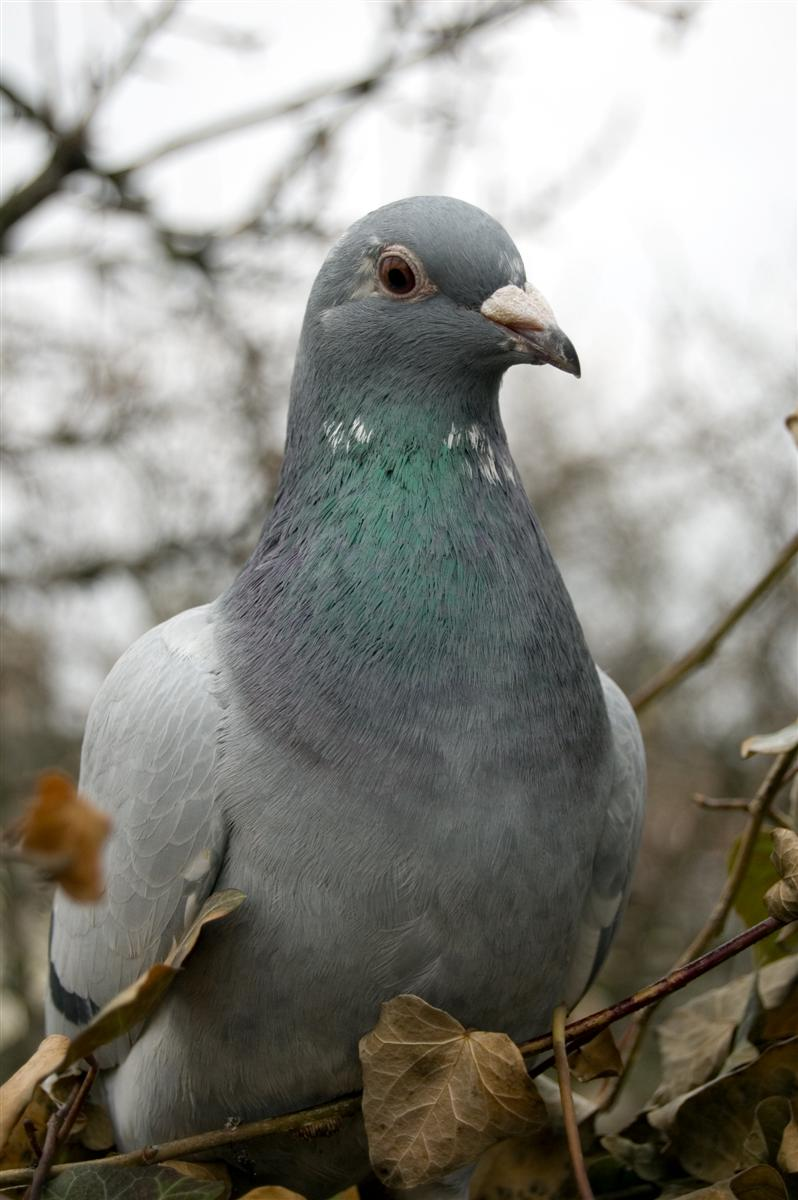
\includegraphics[width=0.7\textwidth]{img/duck.jpeg}
	\caption{A cute duck. Source: Ciwir at pl.wikipedia, CC BY-SA 2.5 <https://creativecommons.org/licenses/by-sa/2.5>, via Wikimedia Commons.}
	\label{fig:duck}
\end{figure}

\subsection{Podrozdział}
Tutaj możemy napisać coś więcej.

\subsubsection{Podpodrozdział}
A tutaj jeszcze więcej.
 % Wprowadzenie + przykładowy rysunek
% =====================================================================
%  Podstawy teoretyczne — przegląd pojęć, definicji i literatury,
%  których czytelnik potrzebuje, żeby zrozumieć resztę pracy.
% =====================================================================
\section{Podstawy teoretyczne}
Lorem ipsum dolor sit amet, consectetur adipiscing elit. Nunc in vehicula est. Proin a justo sagittis, interdum nisl nec, viverra dolor. Etiam at porttitor justo. Ut ut enim nibh. Donec tellus turpis, convallis pulvinar urna sit amet, placerat dignissim felis. Cras tempor eget nunc eu sagittis. Vivamus eget nunc dignissim, lobortis enim quis, sagittis urna. Aenean eget erat dapibus, fermentum arcu sed, lacinia augue. Maecenas velit enim, mollis sed pharetra ac, porta id libero.
     % Podstawy teoretyczne
% =====================================================================
%  Analiza istniejących rozwiązań i technologii — przegląd tego, co już
%  istnieje (biblioteki, narzędzia, podobne prace) z uzasadnieniem
%  wyboru technologii.
%
%  Demonstration deck: listing z kolorowaniem składni (minted, tu Python).
%  minted wymaga kompilacji z -shell-escape i zainstalowanego Pygments —
%  compile.sh załatwia jedno, a pip install Pygments drugie.
% =====================================================================
\section{Analiza istniejących rozwiązań i technologii}
Dzięki swojej prostocie, biblioteka stanowi standard w badaniach dotyczących
głębokiego uczenia oraz w zastosowaniach komercyjnych \cite{Paszke2019pytorch, Paszke2017, Lawson2024}.

\begin{minted}[
    frame=lines,        % Ramka na górze i na dole
    framesep=2mm,       % Odstęp ramki od kodu
    baselinestretch=1.2,% Interlinia dla czytelności
    fontsize=\small,    % Nieco mniejsza czcionka
    linenos             % Numery linii
]
{python}
import torch

# Operacje wykonywane natychmiast, graf budowany dynamicznie
x = torch.tensor([1.0, 2.0, 3.0], requires_grad=True)
y = x.pow(2)        # y.grad_fn = <PowBackward0>
z = y.sum()         # z.grad_fn = <SumBackward0>

print(z.item())     # Wartość dostępna od razu: 14.0

# Propagacja wsteczna przez zbudowany graf
z.backward()
print(x.grad)       # tensor([2., 4., 6.])
\end{minted}
 % Analiza istniejących rozwiązań (listingi)
\section{Projekt i architektura biblioteki}
    % Projekt i architektura
% =====================================================================
%  zestaw przykładów:
%   - wzór \label{eq:indeksliczenie} z odsyłaczem "(str. X)" w tekście,
%   - listing w Rust (minted),
%   - duży rysunek rysowany w TikZ-u (komórki tensorów),
%   - algorytm w pseudokodzie (algorithm2e).
%  Każdy element ma \label, więc można się do niego odwoływać \ref/\pageref.
% =====================================================================
\section{Implementacja podstawowych komponentów} \label{sect:impl}
Tutaj coś piszemy
\subsection{Mechanizm Strides i adresowanie pamięci}
Mapowanie indeksów, wykorzystywane w wielu operacjach, operuje na mechanizmie
kroków (\textit{strides}). Umożliwia to mapowanie wielowymiarowego indeksu, na przykład $(i, j, k)$
na fizyczny adres -- przesunięcie (\textit{offset}) względem początku wektora danych. Obliczenie przesunięcia zostało
ukazany z użyciem wzoru \ref{eq:indeksliczenie} (str. \pageref{eq:indeksliczenie}).
\begin{equation} \label{eq:indeksliczenie}
	\text{offset} = \sum_{d=0}^{D-1} i_d \cdot s_d
\end{equation}
gdzie $i_d$ to indeks w wymiarze $d$, a $s_d$ to wartość kroku (\textit{stride}) dla tego wymiaru. Operacja ta
jest implementowana w metodzie \texttt{physical\_offset}.

\begin{minted}[
    frame=lines,        % Ramka na górze i na dole
    framesep=2mm,       % Odstęp ramki od kodu
    baselinestretch=1.2,% Interlinia dla czytelności
    fontsize=\small,    % Nieco mniejsza czcionka
    linenos             % Numery linii
]
{rust}
pub fn physical_offset(&self, logical_idx: impl AsRef<[usize]>) -> isize {
  let logical_idx = logical_idx.as_ref();
  logical_idx
    .iter()
    .zip(self.strides.iter())
    .fold(0isize, |acc, (&ind, &stride)| acc + ind as isize * stride)
}
\end{minted}


\begin{figure}[h]
	\centering
	\begin{tikzpicture}[every node/.style={font=\scriptsize}]

		% DEFINICJE KOLORÓW
		\definecolor{custorange}{RGB}{255,179,102}
		\definecolor{custpink}{RGB}{255,153,204}
		\definecolor{custcyan}{RGB}{153,255,255}
		\definecolor{custlime}{RGB}{204,255,153}

		% PARAMETRY
		\pgfmathsetmacro{\cellsize}{1.0}
		\pgfmathsetmacro{\depthshift}{1.2}
		\pgfmathsetmacro{\imageshift}{1}
		\pgfmathsetmacro{\imagespace}{6.5}
		\pgfmathsetmacro{\matrixstart}{-6.0}

		% 1. zdjęcia

		\begin{scope}[shift={(\imageshift, 0)}]
			\foreach \h in {0,1} {
					\foreach \w in {0,1,2} {
							\pgfmathsetmacro{\xpos}{\w*\cellsize + \depthshift}
							\pgfmathsetmacro{\ypos}{-\h*\cellsize - \depthshift}

							\fill[custpink, opacity=0.8] (\xpos, \ypos) rectangle ++(\cellsize, -\cellsize);
							\draw[black] (\xpos, \ypos) rectangle ++(\cellsize, -\cellsize);
							\node[font=\tiny] at (\xpos + 0.5*\cellsize, \ypos - 0.5*\cellsize)
							{$i_{1,\w,\h,0}$};
						}
				}

			\foreach \h in {0,1} {
					\foreach \w in {0,1,2} {
							\pgfmathsetmacro{\xpos}{\w*\cellsize}
							\pgfmathsetmacro{\ypos}{-\h*\cellsize}

							\fill[custorange, opacity=0.8] (\xpos, \ypos) rectangle ++(\cellsize, -\cellsize);
							\draw[black] (\xpos, \ypos) rectangle ++(\cellsize, -\cellsize);
							\node[font=\tiny] at (\xpos + 0.5*\cellsize, \ypos - 0.5*\cellsize)
							{$i_{0,\w,\h,0}$};
						}
				}

			\draw[dashed, gray] (0,0) -- (\depthshift, -\depthshift);
			\draw[dashed, gray] (3*\cellsize,0) -- (3*\cellsize+\depthshift, -\depthshift);
			\draw[dashed, gray] (0,-2*\cellsize) -- (\depthshift, -2*\cellsize-\depthshift);
			\draw[dashed, gray] (3*\cellsize,-2*\cellsize) -- (3*\cellsize+\depthshift, -2*\cellsize-\depthshift);

			\node[above, font=\small\bfseries] at (\cellsize + 0.5, 0.3) {Zdjęcie 0 ($B=0$)};
		\end{scope}

		\begin{scope}[shift={(\imagespace, 0)}]
			\foreach \h in {0,1} {
					\foreach \w in {0,1,2} {
							\pgfmathsetmacro{\xpos}{\w*\cellsize + \depthshift}
							\pgfmathsetmacro{\ypos}{-\h*\cellsize - \depthshift}

							\fill[custlime, opacity=0.8] (\xpos, \ypos) rectangle ++(\cellsize, -\cellsize);
							\draw[black] (\xpos, \ypos) rectangle ++(\cellsize, -\cellsize);
							\node[font=\tiny] at (\xpos + 0.5*\cellsize, \ypos - 0.5*\cellsize)
							{$i_{1,\w,\h,1}$};
						}
				}

			\foreach \h in {0,1} {
					\foreach \w in {0,1,2} {
							\pgfmathsetmacro{\xpos}{\w*\cellsize}
							\pgfmathsetmacro{\ypos}{-\h*\cellsize}

							\fill[custcyan, opacity=0.8] (\xpos, \ypos) rectangle ++(\cellsize, -\cellsize);
							\draw[black] (\xpos, \ypos) rectangle ++(\cellsize, -\cellsize);
							\node[font=\tiny] at (\xpos + 0.5*\cellsize, \ypos - 0.5*\cellsize)
							{$i_{0,\w,\h,1}$};
						}
				}

			\draw[dashed, gray] (0,0) -- (\depthshift, -\depthshift);
			\draw[dashed, gray] (3*\cellsize,0) -- (3*\cellsize+\depthshift, -\depthshift);
			\draw[dashed, gray] (0,-2*\cellsize) -- (\depthshift, -2*\cellsize-\depthshift);
			\draw[dashed, gray] (3*\cellsize,-2*\cellsize) -- (3*\cellsize+\depthshift, -2*\cellsize-\depthshift);

			\node[above, font=\small\bfseries] at (\cellsize + 0.5, 0.3) {Zdjęcie 1 ($B=1$)};
		\end{scope}

		\draw[->, ultra thick] (6, -3.5) -- (6, \matrixstart + 0.5)
		node[midway, right] {\texttt{reshape}};

		% 2. MACIERZ

		\begin{scope}[shift={(0, \matrixstart)}]
			\foreach \x/\cellcolor/\idx in {
			0/custorange/i_{0,0,0,0}, 1/custorange/i_{0,1,0,0},
			2/custorange/i_{0,2,0,0}, 3/custorange/i_{0,0,1,0},
			4/custorange/i_{0,1,1,0}, 5/custorange/i_{0,2,1,0},
			6/custcyan/i_{0,0,0,1}, 7/custcyan/i_{0,1,0,1},
			8/custcyan/i_{0,2,0,1}, 9/custcyan/i_{0,0,1,1},
			10/custcyan/i_{0,1,1,1}, 11/custcyan/i_{0,2,1,1}
			} {
			\fill[\cellcolor, opacity=0.8] (\x*\cellsize, 0) rectangle ++(\cellsize, -\cellsize);
			\draw[black] (\x*\cellsize, 0) rectangle ++(\cellsize, -\cellsize);
			\node[font=\tiny] at (\x*\cellsize + 0.5*\cellsize, -0.5*\cellsize) {$\idx$};
			}
		\end{scope}

		\begin{scope}[shift={(0, \matrixstart - 1*\cellsize)}]
			\foreach \x/\cellcolor/\idx in {
			0/custpink/i_{1,0,0,0}, 1/custpink/i_{1,1,0,0},
			2/custpink/i_{1,2,0,0}, 3/custpink/i_{1,0,1,0},
			4/custpink/i_{1,1,1,0}, 5/custpink/i_{1,2,1,0},
			6/custlime/i_{1,0,0,1}, 7/custlime/i_{1,1,0,1},
			8/custlime/i_{1,2,0,1}, 9/custlime/i_{1,0,1,1},
			10/custlime/i_{1,1,1,1}, 11/custlime/i_{1,2,1,1}
			} {
			\fill[\cellcolor, opacity=0.8] (\x*\cellsize, 0) rectangle ++(\cellsize, -\cellsize);
			\draw[black] (\x*\cellsize, 0) rectangle ++(\cellsize, -\cellsize);
			\node[font=\tiny] at (\x*\cellsize + 0.5*\cellsize, -0.5*\cellsize) {$\idx$};
			}
		\end{scope}


	\end{tikzpicture}
	\caption{Przedstawienie zmiany kształtu tensora zbioru dwóch zdjęć na
		reprezentację macierzową bez modyfikacji danych właściwych, a jedynie metadanych.
		Źródło: opracowanie własne}
	\label{fig:conv2dimgreshape}
\end{figure}

\begin{algorithm}[h]
	% UWAGA na kolejność: najpierw \caption, potem \label — inaczej
	% odsyłacz \ref{alg:tensor-iter} pokaże złą numerację.
	\caption{Iterator po tensorze (column-major order)}
	\label{alg:tensor-iter}
	\KwIn{Struktura iteratora $I$}
	\KwOut{Następna wartość lub $\bot$ (brak elementów)}

	\tcp{Struktura TensorIter:}
	\tcp{$I.\text{view}$ -- referencja do tensora}
	\tcp{$I.\text{logical\_pos}$ -- bieżąca pozycja [i₀, i₁, ...]}
	\tcp{$I.\text{finished}$ -- flaga zakończenia}

	\BlankLine
	\If{$I.\text{finished}$}{
		\Return $\bot$
	}

	\tcp{Oblicz fizyczny offset i pobierz wartość}
	$\text{offset} \gets \sum_{d} I.\text{logical\_pos}[d] \cdot I.\text{view}.\text{strides}[d]$\;
	$\text{value} \gets I.\text{view}.\text{data}[\text{offset}]$\;

	\tcp{Inkrementuj pozycję (column-major)}
	$k \gets 0$\;
	\While{$k < |I.\text{view}.\text{shape}|$}{
		$I.\text{logical\_pos}[k] \gets I.\text{logical\_pos}[k] + 1$\;
		\If{$I.\text{logical\_pos}[k] < I.\text{view}.\text{shape}[k]$}{
			\Return $\text{value}$
		}
		$I.\text{logical\_pos}[k] \gets 0$\;
		$k \gets k + 1$\;
	}

	$I.\text{finished} \gets \text{true}$\;
	\Return $\text{value}$
\end{algorithm}

         % Implementacja (wzory, TikZ, algorytmy)
% =====================================================================
%  Badania eksperymentalne — co sprawdzono, jak i z jakim skutkiem:
%  metodyka, zbiory danych, wyniki (tabele/wykresy) i ich interpretacja.
%  Wynik bez interpretacji to nie badanie, tylko screenshot.
%
%  Demonstracja tabeli: tabular + caption + label (label PO caption).
% =====================================================================
\section{Badania eksperymentalne i walidacja biblioteki}\label{sec:badania}
Tutaj coś piszemy...
\subsection{Zbiór XOR}
Zbiór danych XOR składa się z czterech tensorów o wymiarach
$2 \times 1$, zawierających wszystkie możliwe kombinacje wartości
dla funkcji logicznej XOR - co ukazano w tabeli
\ref{tab:xor-dataset}
(str. \pageref{tab:xor-dataset}).
\begin{table}[H]
	\centering
	\caption{Zbiór danych XOR. Źródło: opracowanie własne.}
	\begin{tabular}{|c|c|}
		\hline
		Wejście      & Wyjście \\
		\hline
		$[0, 0]^{T}$ & $[0]$   \\
		$[0, 1]^{T}$ & $[1]$   \\
		$[1, 0]^{T}$ & $[1]$   \\
		$[1, 1]^{T}$ & $[0]$   \\
		\hline
	\end{tabular}

	\label{tab:xor-dataset}
\end{table}
      % Badania eksperymentalne (tabele)
% =====================================================================
%  Podsumowanie i wnioski — co osiągnięto (wnioski odnoszą się do celów
%  z Wstępu!), jakie są ograniczenia i co można zrobić dalej.
%  Rozdział bez numeru, z wpisem w spisie treści.
% =====================================================================
\section*{Podsumowanie i wnioski}
\addcontentsline{toc}{section}{Podsumowanie i wnioski}
\begin{itemize}
	\item Zaprojektowano modułową architekturę biblioteki, umożliwiającą łatwe rozszerzanie
	      przez użytkowników o własne warstwy, optymalizatory, metody inicjalizacji i funkcje straty.
	\item Zaimplementowano od podstaw własny moduł z $n$-wymiarowymi tensorami, obsługującymi
	      mechanizm kroków (\textit{strides}), oraz stosujących podejście typu \textit{zero-copy}
	      (\textit{Copy-on-Write}) -- co pozwalało na uzyskanie wysokiej wydajności oraz efektywnie
	      zarządzanie zasobami. Do operacji mnożenia macierzy skorzystano z zewnętrznej biblioteki.
	\item Stworzono implementacje kluczowych warstw sieci neuronowych -- takich jak warstwy gęste
	      (liniowe), konwolucyjne (Conv2D) z wykorzystaniem własnoręcznie napisanego algorytmu im2col,
	      a także funkcji aktywacji i strat.
	\item W ramach architektury biblioteki opracowano podejście ręcznego różniczkowania -- wymuszającego
	      jawną implementację propagacji wstecznej dla każdego modułu, co pozwala na pełną kontrolę nad przepływem
	      gradientów. Jednocześnie zaimplementowano propagację wsteczną dla warstw wbudowanych.
	\item Stworzono dwa przykładowe programy korzystające z biblioteki -- co pozwoliło na sprawdzenie
	      poprawności jej działania oraz zaprezentowania jej przykładowego użycia.
\end{itemize}
      % Podsumowanie i wnioski

% --- Zamykające ---
% =====================================================================
%  sections/99-tail.tex — bibliografia, spisy i dodatki.
%  Kolejność bloków poniżej odpowiada wymogom wydziału; redagujesz tu
%  głównie Dodatek A (opis tego, co trafia na płytę/archiwum).
% =====================================================================

% Bibliografia: \printbibliography składa wpisy z bibl.bib (biblatex).
% hbadness/hfuzz wyciszają ostrzeżenia o składu — wpisy z DOI i URL-ami
% łamią zasady justowania nieodwołalnie i zaśmiecałyby log.
{
\hbadness=99999
\hfuzz=\maxdimen
\addcontentsline{toc}{section}{Bibliografia}
\printbibliography[title = {Bibliografia}]
}

% Spis rysunków generuje się sam z \caption (styl: tocloft w preambule).
\newpage
\listoffigures

\newpage
\phantomsection % Ważne dla poprawnych linków w PDF (pakiet hyperref)
\addcontentsline{toc}{section}{Spis algorytmów} % Ręczne dodanie wpisu
\listofalgorithms

\pagebreak
\phantomsection % Ważne dla poprawnych linków w PDF (pakiet hyperref)
\addcontentsline{toc}{section}{Dodatek A. Archiwum plików}
\pagestyle{empty}
\section*{Dodatek A. Archiwum plików}
\subsection*{Zawartość archiwum}
W archiwum umieszczono kod źródłowy tego dokumentu (pracy inżynierskiej),
kod źródłowy biblioteki,
przykładów jej wykorzystania oraz pliki wykonywalne na system operacyjny Linux.
Dołączone zostały również karta dyplomowa oraz oświadczenie dot. GenAI.
\subsection*{Uruchamianie przykładów}
Zaleca się uruchamianie programów z poziomu terminala. Wymagany jest procesor
z obsługą AVX512. Należy nadać plikowi uprawnienia do uruchamiania (jeśli ich nie ma):
\begin{verbatim}
chmod +x program
\end{verbatim}
Należy następnie go uruchomić:
\begin{verbatim}
./program
\end{verbatim}
W przypadku chęci samodzielnej kompilacji i uruchomienia przykładów, należy
przejść do katalogu \texttt{mlrs} i użyć menedżera pakietów
\texttt{cargo}:
\begin{verbatim}
cargo run --release --bin [nazwa przykładu]
\end{verbatim}
kompilacja jest gwarantowana w przypadku użycia kompilatora w wersji
\begin{verbatim}
rustc 1.92.0-nightly (b6f0945e4 2025-10-08)
\end{verbatim}
UWAGA: kompilacja jest gwarantowana tylko na systemie linux debian 13 (trixie).
Biblioteka jak i przykłady powinny kompilować się i działać na innych systemach operacyjnych
-- autor nie daje jednak takiej gwarancji.

\newpage
%\pagestyle{plain}
%\pagenumbering{Roman}
%\setcounter{page}{1}
\section*{Dodatek B: Konwencje notacyjne pseudokodu}
\addcontentsline{toc}{section}{Dodatek B: Konwencje notacyjne pseudokodu}

W niniejszej pracy stosuje się notację pseudokodu łączącą elementy programowania funkcyjnego oraz imperatywnego, odpowiadając hybrydowemu charakterowi biblioteki napisanej w języku Rust.

\section*{B.1 Notacja ogólna}

\subsection*{Przypisania i mutacje}
\begin{itemize}
	\item $x \leftarrow \text{wartość}$ -- przypisanie wartości do zmiennej
	\item $L.\texttt{field}$ -- dostęp do pola struktury/obiektu
	\item $\text{list}[i]$ -- indeksowanie tablicy/wektora (numeracja od 0)
	\item $\text{list}.\text{append}(x)$ -- dodanie elementu na koniec listy (mutacja)
\end{itemize}

\subsection*{Struktury kontrolne}
\begin{itemize}
	\item \texttt{ForEach} $x \in X$ -- iteracja po elementach kolekcji
	\item \texttt{While} warunek -- pętla z warunkiem
	\item \texttt{If}/\texttt{eIf}/\texttt{Else} -- instrukcje warunkowe
	\item \texttt{Return} wartość -- zwrócenie wyniku funkcji
\end{itemize}

\section*{B.2 Notacja funkcyjna}

\subsection*{Operacje wyższego rzędu}
\begin{itemize}
	\item $\text{map}(f, xs)$ -- aplikacja funkcji $f$ do każdego elementu listy $xs$
	\item $\text{zipWith}(f, xs, ys)$ -- sparowanie elementów dwóch list i aplikacja funkcji binarnej:
	      $$\text{zipWith}(f, [x_1, x_2, \ldots], [y_1, y_2, \ldots]) = [f(x_1,y_1), f(x_2,y_2), \ldots]$$
	\item $\text{zip}(xs, ys)$ -- sparowanie elementów: $\text{zip}([x_1, x_2], [y_1, y_2]) = [(x_1,y_1), (x_2,y_2)]$
	\item $\text{fold}(f, acc, xs)$ -- redukcja listy z akumulatorem początkowym
\end{itemize}

\subsection*{Równoległość}
\begin{itemize}
	\item $\text{par\_zipWith}(f, xs, ys)$ -- równoległa wersja \texttt{zipWith}
	\item $\text{parallel\_map}(f, xs)$ -- równoległa aplikacja funkcji
	\item Indeks dolny $_{\parallel}$ lub adnotacja \texttt{(równolegle)} -- oznaczenie równoległego wykonania
\end{itemize}

\subsection*{Notacja zbiorowa (list comprehension)}
\begin{itemize}
	\item $[\, f(x) \mid x \in xs, P(x) \,]$ -- lista elementów $f(x)$ dla $x$ spełniających predykat $P$
	\item $\{\, a + b \mid (a,b) \in \text{zip}(xs, ys) \,\}$ -- zbiór sum sparowanych elementów
\end{itemize}

\section*{B.3 Operacje algebraiczne}

\subsection*{Operacje macierzowe}
\begin{itemize}
	\item $A \cdot B$ lub $\text{matmul}(A, B)$ -- mnożenie macierzy
	\item $A^T$ lub $\text{transpose}(A)$ -- transpozycja macierzy
	\item $A \odot B$ lub $\text{elem\_mul}(A, B)$ -- mnożenie element-wise (Hadamard)
	\item $A \oplus \mathbf{b}$ lub $\text{broadcast\_add}(A, \mathbf{b})$ -- dodawanie z rozszerzaniem (broadcasting)
\end{itemize}

\subsection*{Funkcje agregujące}
\begin{itemize}
	\item $\sum_{\text{axis}} A$ lub $\text{sum\_axis}(A, \text{axis})$ -- suma wzdłuż wymiaru
	\item $\text{sum\_rows}(A)$ -- suma wierszy (zwraca wektor kolumnowy)
\end{itemize}

\subsection*{Funkcje aktywacji}
\begin{itemize}
	\item $\sigma(z)$ -- funkcja aktywacji (zazwyczaj sigmoidalna)
	\item $\sigma'(z)$ lub $\text{sigma\_derivative}(z)$ -- pochodna funkcji aktywacji
	\item Aplikacja na macierz: $\sigma(Z)$ oznacza element-wise: $[\sigma(Z)]_{ij} = \sigma(z_{ij})$
\end{itemize}

\section*{B.4 Konwencje specyficzne dla tensorów}

\begin{itemize}
	\item $T.\text{shape}$ -- wektor wymiarów tensora, np. $[C, W, H, B]$
	\item $T.\text{strides}$ -- wektor kroków (strides) w pamięci
	\item $T.\text{data}$ -- surowy wektor danych tensora
	\item $T.\text{iter}()$ -- iterator po elementach w kolejności logicznej
	\item $T.\text{iter\_indices}()$ -- iterator po wielowymiarowych indeksach
	\item $T[idx]$ -- dostęp do elementu przez indeks wielowymiarowy
\end{itemize}

\section*{B.5 Notacje pomocnicze}

\begin{itemize}
	\item $|xs|$ -- długość listy/wektora
	\item $xs \times ys$ -- iloczyn kartezjański (wszystkie pary)
	\item $\text{reversed}(xs)$ -- odwrócenie kolejności elementów
	\item \texttt{// komentarz} lub \tcp{komentarz} -- komentarz wyjaśniający
\end{itemize}

\section*{B.6 Przykłady równoważnych zapisów}

Dla ilustracji, następujące zapisy są równoważne:

\begin{align*}
	\text{zipWith}(+, xs, ys) & \equiv [\, x + y \mid (x,y) \in \text{zip}(xs, ys) \,]   \\
	                          & \equiv \text{map}((x,y) \mapsto x+y, \text{zip}(xs, ys)) \\
	A \cdot B                 & \equiv \text{matmul}(A, B)                               \\
	\sigma(Z)                 & \equiv \text{map}(\sigma, Z) \text{ (element-wise)}
\end{align*}

\section*{B.7 Uwagi implementacyjne}

\begin{itemize}
	\item Operacje oznaczone jako \emph{równoległe} odpowiadają użyciu biblioteki Rayon w implementacji Rust
	\item Notacja funkcyjna (zipWith, map) odpowiada stylowi \emph{iterator chaining} w Rust
	\item Operacje macierzowe są delegowane do biblioteki \texttt{faer}
	\item Wszystkie algorytmy zakładają układ pamięci \emph{column-major} (zerowy wymiar ciągły)
\end{itemize}

\section*{B.8 Obsługa błędów}

W języku Rust funkcje zwracają typ \texttt{Result<T, E>}, będący monadą reprezentującą albo sukces (\texttt{Ok(value)}), albo błąd (\texttt{Err(error)}). W pseudokodzie:

\begin{itemize}
	\item $\text{Ok}(x)$ -- operacja zakończona sukcesem, zwraca wartość $x$
	\item $\text{Err}(e)$ -- operacja nie powiodła się, zwraca błąd $e$
	\item \textbf{panic:} -- nieodwracalny błąd (odpowiednik \texttt{panic!} w Rust)
	\item $\bot$ -- brak wartości (odpowiednik \texttt{None} w \texttt{Option<T>})
\end{itemize}

Algorytmy wykorzystujące walidację wejścia (np. sprawdzanie granic) zwracają \texttt{Result}. Algorytmy, w których błąd jest niemożliwy lub nieistotny, pomijają tę notację dla czytelności.
 % Bibliografia, spisy, dodatki (archiwum płyty itp.)

\end{document}
